% Niveau :      PCSI
% Discipline :  Méca

\begin{exercise}{Bille sur un cerceau}{2}{Sup}
{Mécanique,Ressort}{lelay}


\begin{questions}
    \questioncours Donner l'énergie potentielle correspondant à un ressort de raideur $k$ et de longueur à vide $\ell_0$.

\begin{EnvUplevel}
On considère une bague pesante de masse $m$ glissant sans frottement sur un cercle de rayon $R$, comme sur le schéma ci-dessous.

\begin{center}
    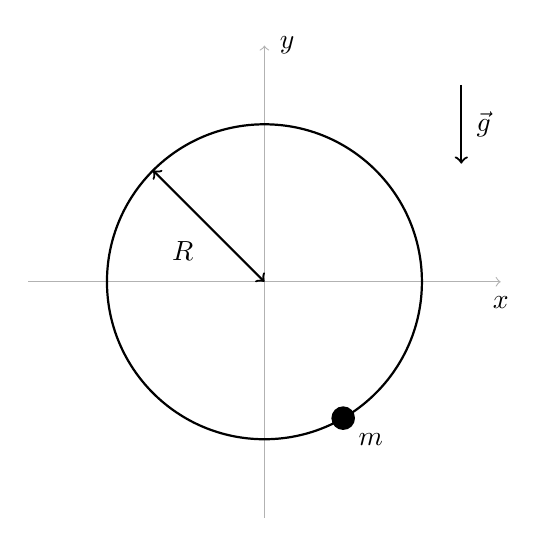
\begin{tikzpicture}
    
    \draw[->, black!30] (-3, 0) -- (3, 0);
    \draw (3,0) node[below=2pt] {$x$};
    
    \draw[->, black!30] (0, -3) -- (0, 3);
    \draw (0,3) node[right=2pt] {$y$};
    
    
    \draw[color=black, thick](0,0) circle (2);
    
    \fill[black] (0.5*2,-0.866*2) circle (0.15);
    \draw (0.5*2,-0.866*2) node[below right=2pt] {$m$};
    
    \draw[<->, thick] (0,0) -- (-0.707*2,0.707*2);
    \draw (-0.707*1,0.707*1) node[below left=2pt] {$R$};
    
    \draw[->, thick] (2.5, 2+0.5) -- (2.5, 2-0.5);
    \draw (2.5,2) node[right=2pt] {$\vec{g}$};
    
    \end{tikzpicture}
\end{center}

\end{EnvUplevel}
    
    \question Donner l'équation du mouvement de la bague. À quel système cette équation vous fait-elle penser ?
    \question En supposant la bille proche du bas du cerceau, quelle approximation permet de linéariser l'équation précédente ? Donner l'équation linéarisée et la famille de solutions correspondante.
    \uplevel{On ajoute maintenant un ressort de raideur $k$ et de longueur à vide $2R$ reliant la bague au point le plus haut du cerceau, comme sur le schéma ci-dessous.}

\begin{center}
    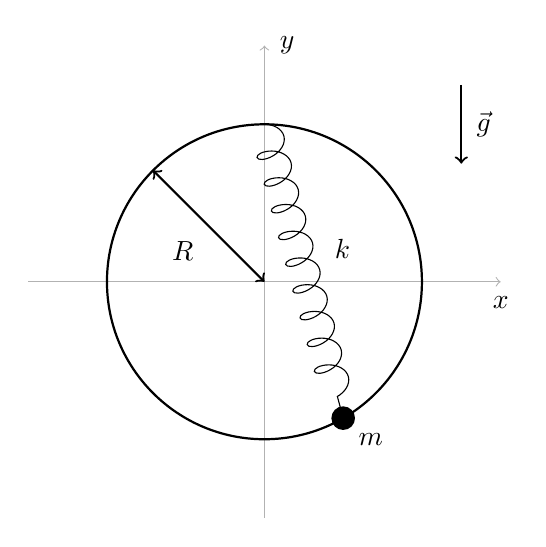
\begin{tikzpicture}
    
    \draw[->, black!30] (-3, 0) -- (3, 0);
    \draw (3,0) node[below=2pt] {$x$};
    
    \draw[->, black!30] (0, -3) -- (0, 3);
    \draw (0,3) node[right=2pt] {$y$};
    
    \draw[color=black, thick](0,0) circle (2);
    
    \fill[black] (0.5*2,-0.866*2) circle (0.15);
    \draw (0.5*2,-0.866*2) node[below right=2pt] {$m$};
    
    \draw[<->, thick] (0,0) -- (-0.707*2,0.707*2);
    \draw (-0.707*1,0.707*1) node[below left=2pt] {$R$};
    
    \draw[->, thick] (2.5, 2+0.5) -- (2.5, 2-0.5);
    \draw (2.5,2) node[right=2pt] {$\vec{g}$};
    
    \draw[decoration={aspect=0.6, segment length=10, amplitude=2mm,coil},decorate] (0,2) -- (0.5*2,-0.866*2);
    \draw (0.7,0.1) node[above right=2pt] {$k$};
    
    \end{tikzpicture}
\end{center}
    \question Donner la nouvelle équation du mouvement de la bague.
    \question En supposant la bille proche du bas du cerceau, développer l'équation jusqu'au premier terme non linéaire. On prendra $k = \frac43 \frac{mg}{R}$.
    \question Quel est l'intérêt de ce dispositif ?

\end{questions}

\end{exercise}

\begin{solution}

\begin{questions}
    \questioncours $E_p = \frac12 k (\ell-\ell_0)^2$
    \question Même dérivation que le pendule (par l'énergie ou la dynamique), on trouve une équation de pendule
    $$ \ddot \theta + {\omega_0}^2\sin \theta = 0$$
    avec $\omega_0 = \sqrt{g / R}$
    \question Équation d'oscillateur harmonique de pulsation $\omega_0$
    \uplevel{On ajoute maintenant un ressort de raideur $k$ et de longueur à vide $\ell_0 = 2R$ reliant la bague au point le plus haut du cerceau, comme sur le schéma ci-dessous.}

    \question 2 possibilités : 
    \begin{itemize}
        \item Rajouter une force de norme $k |\ell - 2R|$. L'angle rajoute un facteur $\sin(\frac\theta2)$.
        
        \item Travailler avec l'énergie mécanique, qui est
    \end{itemize}
    \begin{align*}
    E_m &= E_c + E_{p,g} + E_{p, r} \\
        E_m &= \frac12m R^2\dot{\theta}^2 + mgh + \frac12 k (\ell - 2R)^2
    \end{align*}
    Avec la hauteur $h = - R\cos \theta$ et la longueur du ressort $\ell = 2R \cos(\theta/2)$, d'où
    \begin{align*}
        E_m &= \frac12m R^2\dot{\theta}^2 - mgR\cos\theta + kR (\cos(\theta/2) - 1)^2 \\
        \dd{E_m}/\dd{t} = 0 &= mR^2 \ddot\theta + mgR\sin\theta + 2 kR \sin(\frac{\theta}2)\qty(1 - \cos(\theta/2))
    \end{align*}
    À la fin on doit retomber sur l'équation de la dynamique :
    \begin{align*}
        \ddot{\theta} + \frac{g}{R} \sin\theta + \frac{2k}{m} \sin(\frac{\theta}2)\qty(1 - \cos(\frac{\theta}2)) &= 0
    \end{align*}
    \question À l'ordre 1 le terme supplémentaire ne contribue pas (on a tj un oscillateur harmonique de pulsation $\sqrt{g/L}$). Surprise, les termes d'ordre 3 s'annulent ! Il reste des termes d'ordre 5.
    \question On a réussi à compenser la première non linéarité, on a donc des oscillations plus isochrones

\end{questions}
\end{solution}